\documentclass[xcolor=dvipsnames,hyperref={pdfpagelabels=false}]{beamer}

\usetheme{Berkeley}

\let\Tiny=\tiny

\newcommand{\bi}{\begin{itemize}}
\newcommand{\ei}{\end{itemize}}
\newcommand{\be}{\begin{enumerate}}
\newcommand{\ee}{\end{enumerate}}
\newcommand{\I}{\item}
\newcommand{\f}{\frame}
\newcommand{\ft}{\frametitle}

\title{Status of the Offline Software}
\subtitle{GlueX Collaboration Meeting}
\author[M.\ Ito]{Mark M.\ Ito}
\date{October 6, 2011}
\institute[JLab]{Jefferson Lab}

\begin{document}

\f{\titlepage}

\f{
\bi
\I Volatile disk
  \bi
  \I ``scratch'' disk available from Batch Farm at JLab
  \I up to 40 TB
  \I could be used as staging disk before writing to tape
  \I in addition to 9 TB of work disk space
  \ei
\I Resource Management
  \bi
  \I need scheme to deal with large, non-run dependent data files
  \I e. g., magnetic field maps, material maps
  \I Dmitry proposed conceptual design
  \I uniform interface
  \I local caching
  \ei
\ei
}

\f{
\ft{Whither the CCDB?}
\bi
\I Beta release in the wild since November
  \bi
  \I functioning, full-featured shell interface
  \I JANA compatibility demonstrated
  \ei
\I Not much activity testing it
\I Not much activity documenting it
\I Deployment issues not fully implemented
\I Off-site accessible MySQL mirror: agreement in principle with IT Division
\I Not the default calibration repository yet
\ei
}

\f{
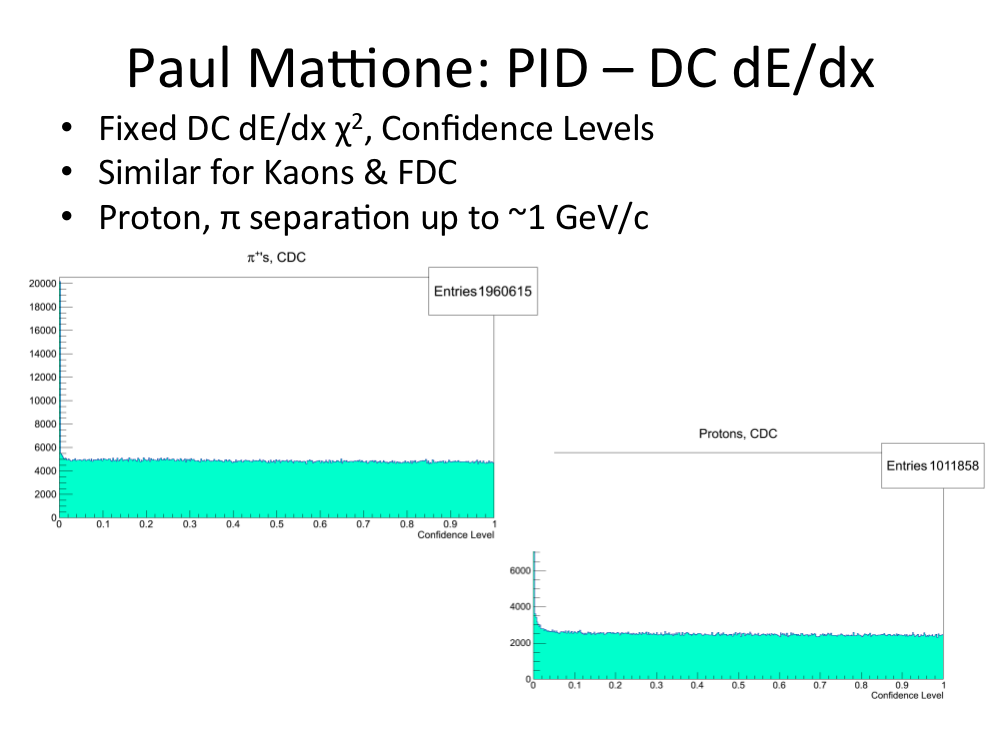
\includegraphics[height=3.0in]{Mattione_dedx.png}
}

\f{
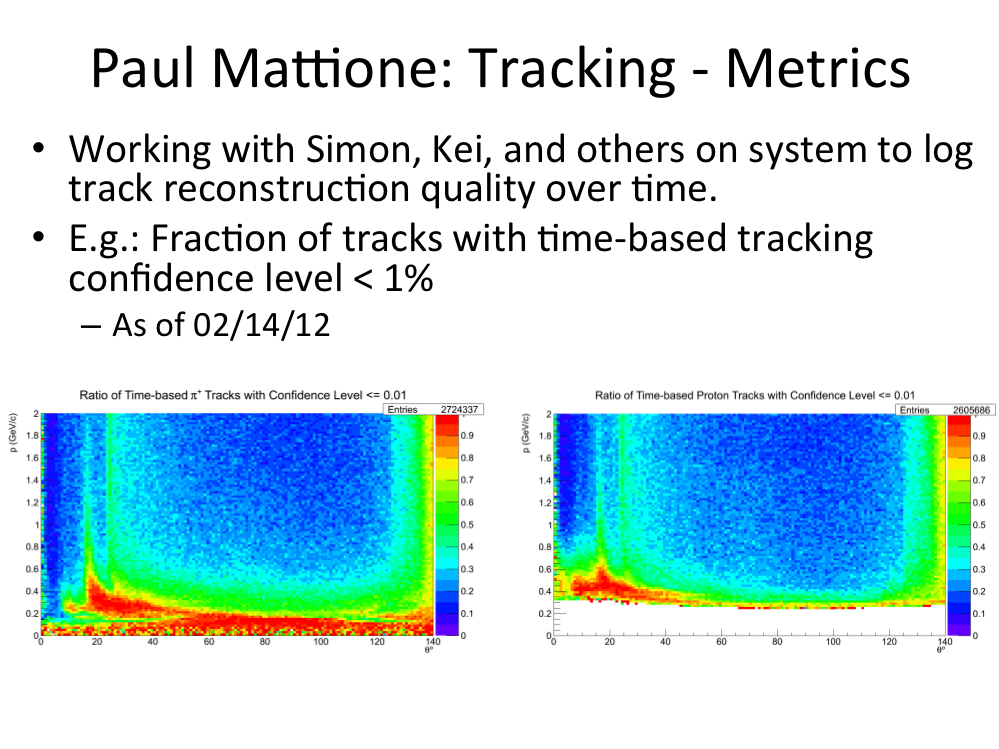
\includegraphics[height=3.0in]{Mattione_metrics.png}
}

\f{
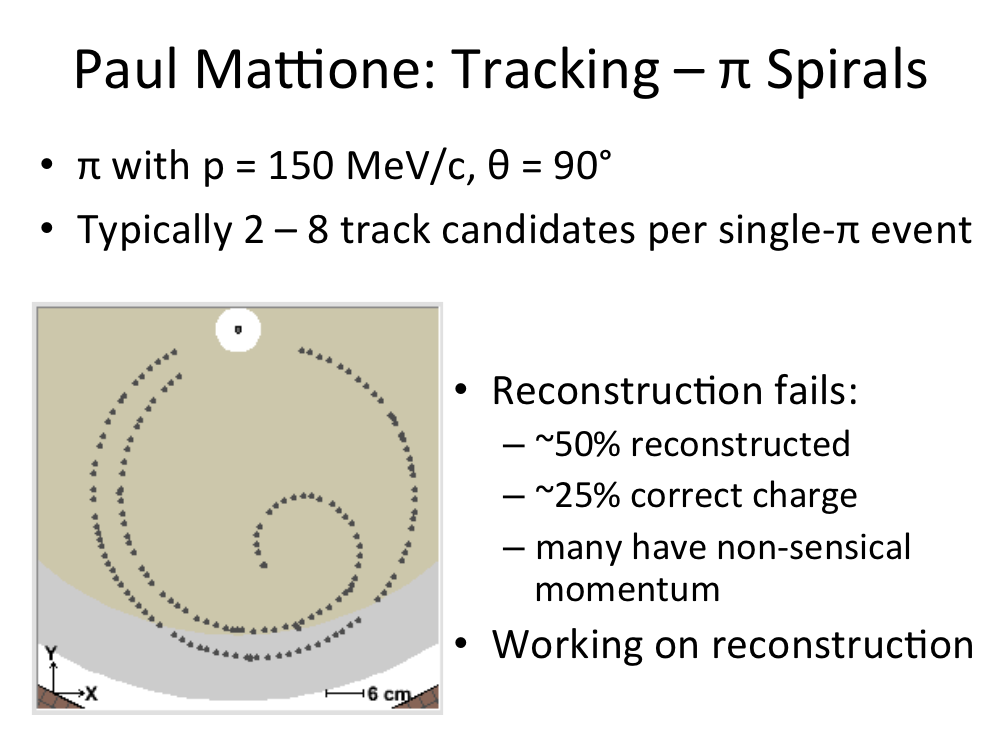
\includegraphics[height=3.0in]{Mattione_spirals.png}
}

\f{
\ft{Miscellaneous Topics}
\bi
\I Beni reported increase in number of photons in the b1pi job last November.
\I Heard a report from Gagik Gavalian on CLARA-based DST analysis system using data in HCF5 format.
\I Memory explosion problem found and fixed.
  \bi
  \I was causing irritation of sysadmin personnel at grid sites
  \I problem with never-ending propagation of tracks at 90 degrees with hits in FDC
  \I fixed in sim-recon-2012-01-27
  \ei
\ei
}

\end{document}

%%% end of latex file %%%%
